% Define document class. Important.
\documentclass[a4paper,twoside,openright]{report}

\usepackage{acronym}

% Margener
%\setlength{\evensidemargin}{1cm}
%\setlength{\oddsidemargin}{1cm}

% Set up encoding. Latin1 since UTF-8 is fuckably difficult to work with.
\usepackage[utf8x]{inputenc}
%\usepackage[T1]{fontenc}
% Load up bibliography.
\usepackage[authoryear]{natbib}
\setcitestyle{numbers,square}
% Bibliography style.
\bibliographystyle{plainnat}

% Algorithm support.
\usepackage{algorithmic}
\usepackage{algorithm2e}
\usepackage{subfig}
\usepackage{amsmath}
\usepackage{amsfonts}


% Image frames.
\setlength{\fboxsep}{0pt}
\setlength{\fboxrule}{0.5pt}

% Also, images.
\usepackage{graphicx}

% tabeller der strækker sig over flere sider
\usepackage{longtable}

% flere tabel-muligheder
\usepackage{multirow}

% bedre enumerate
\usepackage{enumitem}

% Todo notes here and there.
% write instead for disable: \usepackage[disable]{todonotes}
\usepackage[disable]{todonotes}

% Forbedrede floats.
\usepackage{float}
\usepackage{rotating}

% Special symbols availability.
\usepackage{amssymb}

\usepackage{textcomp}

% CODE %
\usepackage{listings}
\usepackage[scaled]{beramono} % Better font for listings
\usepackage{color}
\definecolor{gray}{rgb}{0.4,0.4,0.4}
\definecolor{darkblue}{rgb}{0.0,0.0,0.6}
\definecolor{cyan}{rgb}{0.0,0.6,0.6}
\lstset{
  tabsize=4,
  breaklines=true,
  numbers=left,
  captionpos=b,
  stepnumber=1,
  numbersep=10pt,
  showstringspaces=false,
  basicstyle=\footnotesize,
}% Neat-o referencer...o.
\usepackage{bookmark,hyperref}
\usepackage{nameref}

% hack fra nettet.
% http://tex.stackexchange.com/questions/1230/reference-name-of-description-list-item-in-latex
\makeatletter
\let\orgdescriptionlabel\descriptionlabel
\renewcommand*{\descriptionlabel}[1]{
  \let\orglabel\label
  \let\label\@gobble
  \phantomsection
  \edef\@currentlabel{#1}
  %\edef\@currentlabelname{#1}
%  \let\label\orglabel
  \orgdescriptionlabel{#1}
}
\makeatother
% Rettehak. Meget lettere end \checkmark
\newcommand{\yes}{\checkmark}

\pagenumbering{arabic} % Ensure page numbering in our desired form.

% New command for two figures, side by side.
\newcommand{\twofigs}[6]
{
	\begin{figure}[H]
		\begin{minipage}[b]{0.5\columnwidth}
		\centering\fbox{\includegraphics[width=0.8\columnwidth]{img/#1}}\caption{#2\label{#3}}
		\end{minipage}
		\hspace{0.5cm}
		\begin{minipage}[b]{0.5\columnwidth}
		\centering\fbox{\includegraphics[width=0.8\columnwidth]{img/#4}}\caption{#5\label{#6}}
		\end{minipage}	\end{figure}
}

% Sørg for at paragrafplads ikke spildes.
\raggedbottom
\usepackage[titletoc]{appendix}

% Package til at regne forskellen ud mellem 2 labels
\usepackage{refcount}
\newcommand{\pagedifference}[2]{\number\numexpr\getpagerefnumber{#2}-\getpagerefnumber{#1}\relax}

% Opsætning af autoref%
\def\figureautorefname{Figure}
\def\tableautorefname{Table}
\def\chapterautorefname{Chapter}
\def\sectionautorefname{Section}
\def\subsectionautorefname{Subsection}

%Ingen indentering
\setlength{\parindent}{0mm}


\begin{document}
\acrodef{crud}[CRUD]{Create, Read, Update, Delete}
\acrodef{api}[API]{Application Programming Interface}
\acrodef{json}[JSON]{JavaScript Object Notation}
\acrodef{xml}[XML]{Extensible Markup Language}
\acrodef{api}[API]{Application Programming Interface}
\acrodef{cat}[CAT]{Category Administration Tool}
\acrodef{lamp}[LAMP]{Linux, Apache2, MySql and PHP}
\acrodef{giraf}[GIRAF]{Graphical Interface Resources for Autistic Folk}
\acrodef{oha}[OHA]{Open Handset Alliance}
\acrodef{gui}[GUI]{Graphical User Interface}
\acrodef{json}[JSON]{JavaScript Object Notation}
\acrodef{foss}[FOSS]{Free and Open-Source Software}
\acrodef{ui}[UI]{User Interface}

\pagestyle{empty}

\thispagestyle{empty}
\begin{flushright}
\vspace{3cm}

\phantom{hul}

\phantom{hul}

\phantom{hul}

\textsl{\Huge WASTELAND}\\ \vspace{0.3cm}
\textsl{\Huge - A GIRAF Database} \vspace{0.5cm}

\rule{13cm}{3mm} \\ \vspace{1.5cm}
\vspace{1cm}

%Insert image here!
%\includegraphics[width=1.0\textwidth]{img/image} 

\vspace{1.5cm} 
\textsc{\Large P6 Project \\
Group SW603 \\
Department of Computer Science\\
Aalborg University\\
Some date 2013\\}
\end{flushright}

\cleardoublepage

% Dette er LaTeX-versionen af titelbladet for tek-nat-basis-rapporter 2004 efterår
% Filen kræver:
% Universitetets logo:  aau-logo.png (for LaTeX) eller aau-logo.ps (for LaTeX)
% Synopsis: En fil ved navn synopsis.tex

% Udarbejdet af: Hans Hüttel (hans@cs.auc.dk) 21. maj 2003
% Rettet af Morten Christophersen (mortench@tnb.aau.dk) 30. nov 2004(Ændret til nyt design 2004 efterår)

\phantomsection
\pdfbookmark[0]{Titlepage}{titlepage}
\thispagestyle{empty}
%\begin{titlepage}
\begin{nopagebreak}
{\samepage 
\begin{tabular}{r}
\parbox{\textwidth}{  \raisebox{11mm}{
\includegraphics[height=1.2cm]{img/aau-logo-1.png}}\\
\hfill \parbox{8cm}{\begin{tabular}{l} %4.90
{\small \textbf{Institut for Computer Science}}\\
{\small Selma Lagerlöfs Vej 300} \\
{\small 9220 Aalborg Ø} \\
{\small Phone 99 40 99 40} \\
{\small Fax 99 40 97 98} \\
{\small http://www.cs.aau.dk/}
\end{tabular}}}

\end{tabular}

\begin{tabular}{cc}
\parbox{7cm}{
\begin{description}

\item { Title:} 

WASTELAND - A GIRAF Database \\
  
\item { Theme:} 

Developing Complex Software Systems

\end{description}

\parbox{8cm}{

\begin{description}
\item { Project period:}\\
   6th semester 2013 SW
  \hspace{4cm}
\item { Project group:}\\
  SW603F13
  \hspace{4cm}
\item { Group members:}\\
Barbara Flindt\\
Hilmar Laksá Magnussen \\
Jeppe Blicher Tarp \\
Simon Jensen\\
  \hspace{2cm}
\item { Counselor:}\\
 Katja Hose\\
  
\end{description}
}
\begin{description}
\item { Circulation: 6 }
\item { Number of pages: 103 } 
\item { Number of Appendices: 3} 
\item { Finished } 4th of June 2013
\end{description}
\vfill } &
\parbox{7cm}{
  \vspace{.15cm}
  \hfill 
  \begin{tabular}{l}
  { Abstract:}\bigskip \\
  \fbox{
    \parbox{7cm}{\bigskip
     {\vfill{\small We describe the design and implmentation of a central server application for the GIRAF system with a database, an API for communication and synchronization between the central database and a local counterpart on an Android device. This is done in the context of a multiproject consisting of 8 groups, all working on various aspects of the GIRAF system. We end up with a working implementation and describe future work and tips for future students working on top of this project.
     \bigskip}}
     }}
   \end{tabular}}
\end{tabular}}
\\ \\ \\ \\ \\ \\ \\
\noindent{\footnotesize{\textit{Rapportens indhold er frit tilgængeligt, men offentliggørelse (med kildeangivelse) må kun ske efter aftale med forfatterne.}}}
\end{nopagebreak}
%\end{titlepage}

\cleardoublepage

\listoftodos
\chapter*{Preface}



\cleardoublepage
\pdfbookmark{Table of Contents}{toc}
\tableofcontents
\cleardoublepage
\pagestyle{plain}

%input main content here
\chapter{Common Chapter}
This is where the common chapter will go.
	
\chapter{User Manual}

\emph{(Chapter introduction goes here)}
\chapter{User Manual}

\emph{(Chapter introduction goes here)}
\chapter{User Manual}

\emph{(Chapter introduction goes here)}
\chapter{User Manual}

\emph{(Chapter introduction goes here)}
\chapter{User Manual}

\emph{(Chapter introduction goes here)}
\chapter{User Manual}

\emph{(Chapter introduction goes here)}
\chapter{User Manual}

\emph{(Chapter introduction goes here)}
\chapter{User Manual}

\emph{(Chapter introduction goes here)}

\bookmarksetup{startatroot}% dette skulle stoppe part, så conclusion får indryk. Problemet i skrivende øjeblik er at chapters har samme indryk uafhængigt af parts
\addtocontents{toc}{\bigskip}%laver ekstra mellemrum

\cleardoublepage
\begin{appendices}
\chapter{API Documentation}\label{app:api}
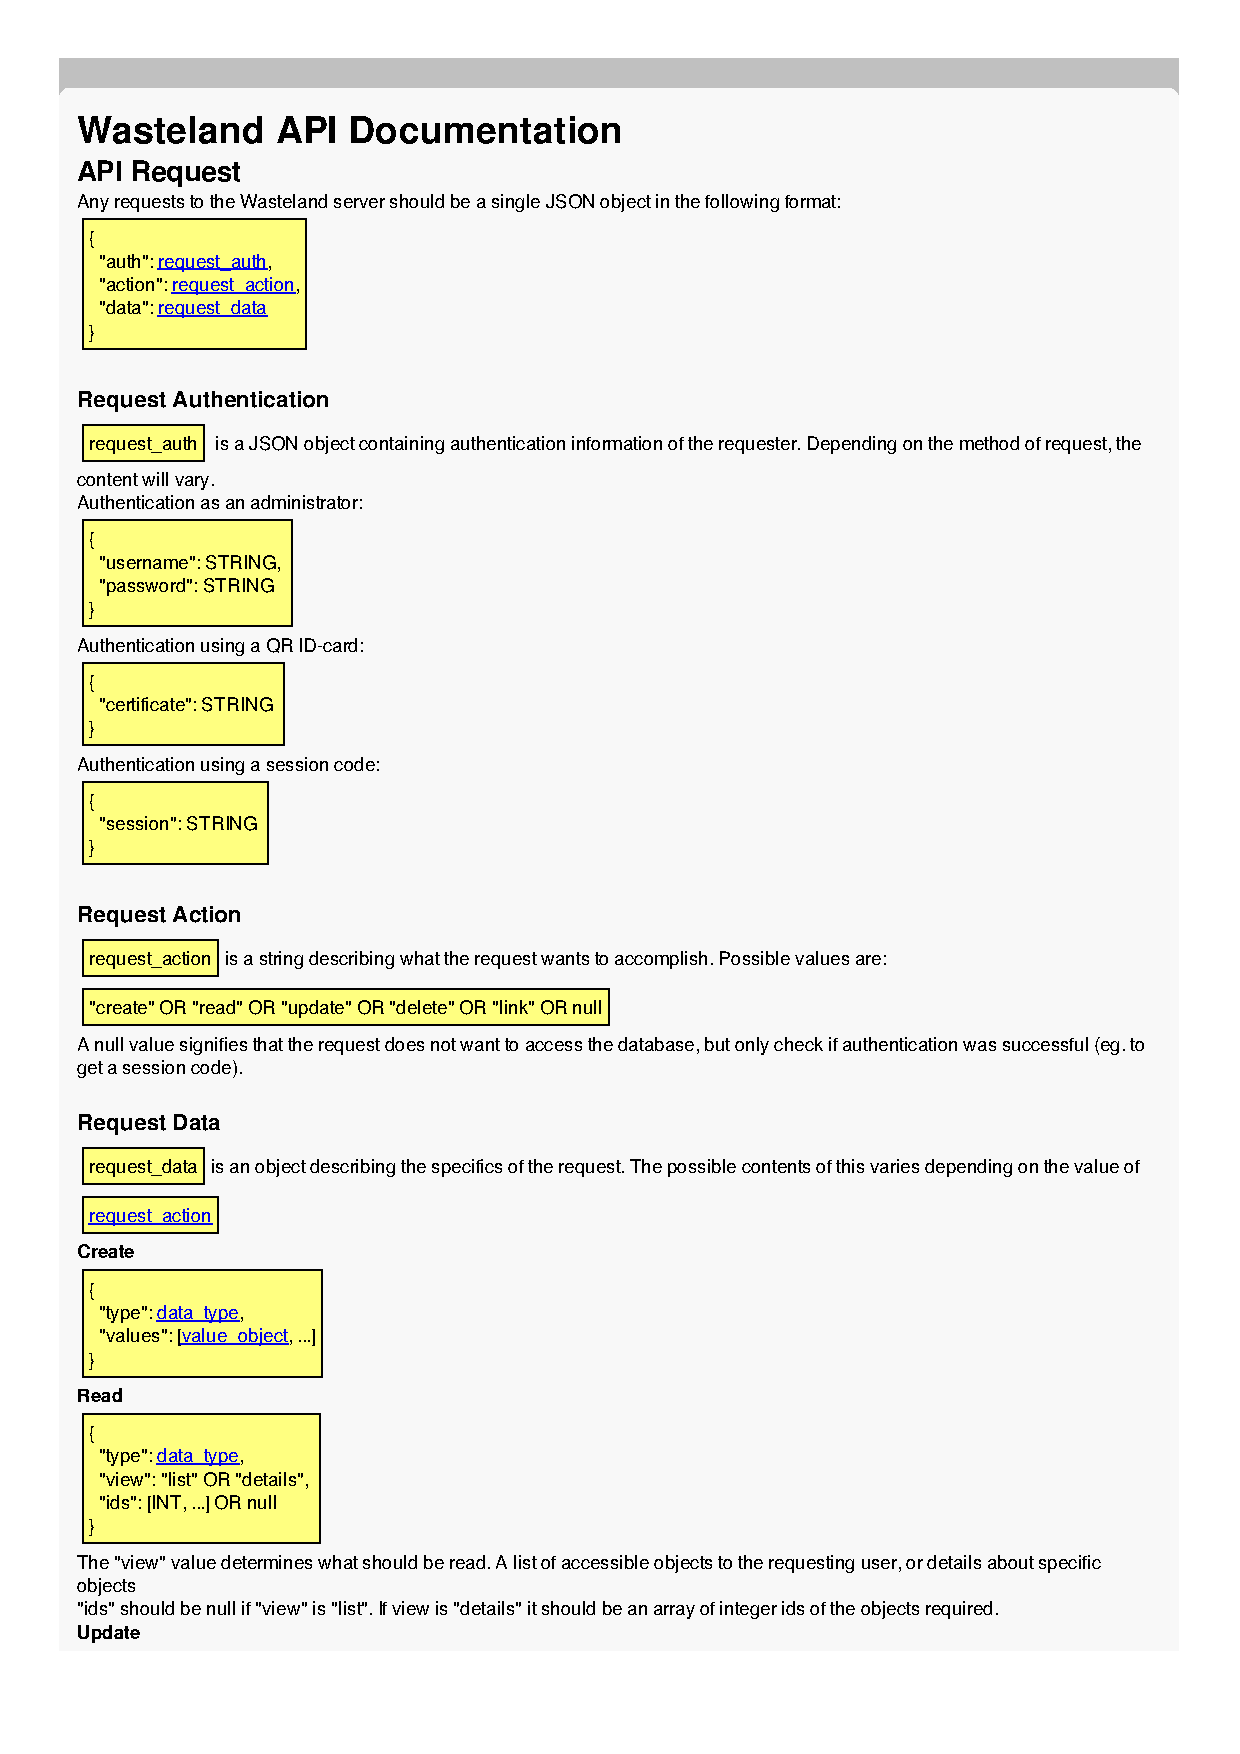
\includepdf[pages={1}]{img/appendix_api}
\includepdf[pages={2}]{img/appendix_api}
\includepdf[pages={3}]{img/appendix_api}
\includepdf[pages={4}]{img/appendix_api}
\includepdf[pages={5}]{img/appendix_api}
\end{appendices}
\cleardoublepage
\pdfbookmark{Bibliography}{bib}
\bibliographystyle{plain}
\bibliography{bib/bibliography}

\end{document}
